\documentclass[a4paper, 12pt, twoside]{report}

\usepackage{physics, amsmath, amsfonts, systeme}
\usepackage{tcolorbox}
\usepackage{enumitem}
\usepackage{hyperref}
\usepackage{graphicx}
\graphicspath{ {./ch1} }
\hypersetup{
        colorlinks=true,
                linkcolor=black,
                urlcolor=blue,
}

\usepackage{geometry}
\geometry{
        top=2cm,
                bottom=2cm,
                left=2cm,
                right=3cm,
                headheight=17pt,
                includeheadfoot,
}

\usepackage{fancyhdr, lastpage}
\pagestyle{fancy}
\fancyhf{}
\lhead{Mettere icona GitHub}
\rhead{ Relatività Ristretta }
\cfoot{Pagina \thepage\ di \pageref{LastPage}}
\renewcommand{\headrulewidth}{1.0pt}

\usepackage{etoolbox}
\patchcmd{\chapter}{\thispagestyle{plain}}{\thispagestyle{fancy}}{}{}

\title{Cinematica Relativistica}
\author{Pietro Garofalo}
\date{\today}


\begin{document}

\maketitle
\newpage
\tableofcontents

\chapter{Le trasformazioni di Lorentz }
In relatività le trasformazioni di Galileo sono sostituite dalle trasformazioni di Lorentz, prima di vederle nel dettaglio bisogna ricordarsi 
che le grandezze che ci interessano non sono più i semplici vettori ma i \textbf{ quadrivettori contravarianti } che definiamo nel seguente modo :
\begin{center}
        
        $ \vectorbold{X^{\mu}} = \begin{pmatrix} ct\\ \va{x} \end{pmatrix} $

\end{center}
Tale notazione evidenzia come i quadrivettori siano divisi in una parte temporale ( la prima componente ) e componenti spaziali ( vettore tridimensionale ), 
tali quaterne di valori trasformano, nel passaggio da un sistema di riferimento ad un altro, tramite le trasformazioni di Lorentz. \\
La metrica dei quadrivettori non è la metrica Euclidea bensì quella di \textbf{Minkowski}, se definiamo infatti due quadrivettori 
\begin{align*}
        \vectorbold{A^{\mu}} = \begin{pmatrix} a_0\\a_1\\a_2\\a_3\end{pmatrix}
        \
        \vectorbold{B^{\mu}} = \begin{pmatrix} b_0\\b_1\\b_2\\b_3\end{pmatrix}
\end{align*}
Allora il prodotto fra i due si definisce come :
\begin{align*}
        \vectorbold{A^{\mu}}\vdot\vectorbold{B_{\mu}} = a_0b_0 - a_1b_1 - a_2b_2 - a_3b_3
\end{align*}
dove $\vectorbold{B_{\mu}}$ non è altro che il \textbf{quadrivettore covariante} ossia il quadrivettore contravariante ma con il segno della parte spaziale opposto .\\
D'ora in avanti indicheremo $\vectorbold{X} \equiv \vb{X^{\mu}} $.
\newpage

\section{Trasformazione delle coordinate}
Supponiamo di avere un sistema di riferimento $\mathbb O$ fermo ( sistema del laboratorio ) e un sistema $\mathbb O^{'} $ in movimento 
con velocità V come in figura.\\

\begin{figure}[!h]
        \centering 
        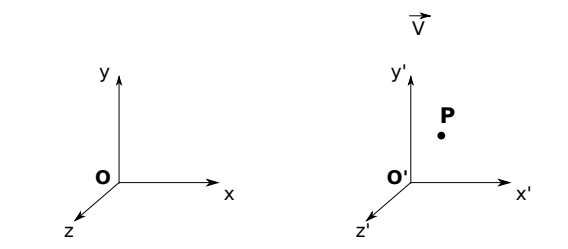
\includegraphics[scale=0.8]{SistemaRiferimento}
        \caption{Sistemi di riferimento}
\end{figure}
Indichiamo con $\vb{X}$ il quadrivettore posizione del punto \textbf{P} rispetto a $\mathbb O$ e $\vb{X^\prime}$ rispetto a $\mathbb O^\prime$, le coordinate di 
$\vb{X^\prime}$ si trovano rispetto alle coordinate misurate in $\mathbb O^\prime$ nel seguente modo : 
\begin{align*}
        \vectorbold{X^\prime} = \vb{\Lambda^{\mu}_{\nu}} \vb{X} 
\end{align*} 
dove $\vb{\Lambda^{\mu}_{\nu}}$ rappresenta la matrice della trasformazione di Lorentz lungo asse x data da : 
\begin{align*}
        \vb{\Lambda^{\mu}_{\nu}} = \begin{pmatrix} \gamma & -\gamma\beta & 0 & 0 \\ -\gamma\beta & \gamma & 0 & 0 \\ 0 & 0 & 1 & 0 \\ 0 & 0 & 0 & 1 \end{pmatrix} \tag*{$\beta = \frac{V}{c}$ \ $\gamma = \frac{1}{\sqrt{1-\beta^2}}$}
\end{align*}
si ottiene quindi il seguente sistema : 
\begin{equation*}
\left\{ \begin{aligned}
        ct^{\prime}&=\gamma(ct - \beta x) \\
        x^{\prime}&= \gamma( x - ct\beta ) \\
        y^{\prime}&= y \\
        z^{\prime} &= z
  \end{aligned}
  \right.
\end{equation*}
\begin{tcolorbox}[colback=red!5!white,colframe=red!50!black,title=ATTENZIONE !]
Se il cambio di sistema di riferimento si fa dal sistema in moto al sistema di riferimento del laboratorio allora $\beta$ cambia di segno 
\end{tcolorbox}
\newpage
\section{Trasformazione delle velocità}
Per capire bene le trasformazioni delle velocità conviene vedere un esercizio.\\
\begin{center}\textbf{Esercizio  }\end{center} 
Un uomo in automobile viaggia ad una velocità di $\frac{3}{4}c$, viene inseguito da un'altra automobile che va alla velocità di $\frac{1}{2}c$ 
la quale spara un proiettile che va alla velocità di $\frac{1}{3}c$.
Il proiettile raggiunge l'auto ? \\
\begin{center}\textbf{Soluzione}\end{center}
La questione è tutta basata sulle trasformazioni delle velocità in relatività, le troveremo tramite le trasformazioni di Lorentz viste prima, 
un commento prima di trovarle : 
\\
\begin{tcolorbox}[colback=red!5!white,colframe=red!50!black,title=ATTENZIONE !]
Bisogna capire bene i sistemi di riferimento, nel nostro caso stiamo osservando le macchine che corrono, noi siamo il laboratorio ( sistema fermo )
il problema è che la velocità del proiettile è calcolata nel sistema di riferimento in moto ( ossia la macchina che spara ), il gioco è tutto quì : 
trasformare la velocità del proiettile dal sistema di riferimento in moto a quello del laboratorio . 
\end{tcolorbox}
Partiamo dalla trasformazione di Lorentz per la posizione, come al solito identifichiamo con $x^{\prime}$ le coordinate del sistema di riferimento in moto : 
\begin{equation*}
\left\{ \begin{aligned}
                ct&=\gamma(ct^{\prime} + \beta x^{\prime}) \\
        x&= \gamma( x^{\prime} + ct\beta ) \\
        y&= y^{\prime} \\
        z&= z^{\prime}
  \end{aligned}
  \right.
\end{equation*}
Notare come c'è il cambio di segno dovuto al fatto che passiamo da sistema in moto a quello del laboratorio. \\
Passiamo ora agli infinitesimi : 
\begin{equation*}
        \left\{ \begin{aligned}
                        c\dd{t} &= \gamma c\dd{t^{\prime}} + \beta\gamma\dd{x^{\prime}} \\
                        \dd{x} &= \gamma\dd{x^{\prime}} + c\gamma\beta\dd{t^{\prime}} \\
                        \dd{y} &= \dd{y^{\prime}} \\
                        \dd{z} &= \dd{z^{\prime}} \\
                \end{aligned}
                \right.
\end{equation*}
Dividiamo ora ciascuna componente per $\dd{t}$ la cui espressione l'abbiamo ricavata sopra, dividiamo poi numeratore e denominatore per $\dd{t^{\prime}}$, sostiuiamo $ \frac{\dd{x^{\prime}}}{\dd{t^{\prime}}} \equiv \dd{v^{\prime}_{x}} $ eccetera, inoltre $\beta \equiv \frac{V}{c}$ 
dove V è la velocità del proiettile nel sistema in moto, si ottiene : 
\newpage
\begin{equation*}
        \left\{ \begin{aligned}
                        \frac{\dd{x}}{\dd{t}} &\equiv v_{x}&= \frac{\gamma v^{\prime}_{x} + \gamma V}{\gamma(c + \frac{V}{c}v^{\prime}_{x})} \\
                        \frac{\dd{y}}{\dd{t}} &\equiv v_{y}&= \frac{v^{\prime}_{y}}{\gamma(c + \frac{V}{c}v^{\prime}_{x})} \\
                        \frac{\dd{z}}{\dd{t}} &\equiv v_{z}&= \frac{v^{\prime}}{\gamma(c + \frac{V}{c}v^{\prime}_{x})}
            \end{aligned}
            \right.
\end{equation*}
Abbiamo così ottenuto le trasformazioni delle velocità : 
\begin{tcolorbox}[colback=red!5!white,colframe=red!50!black,title=ATTENZIONE !]
        \begin{equation*}
                \left\{ \begin{aligned}
                                v_{x} &= \frac{V + v^{\prime}_{x}}{c + \frac{V}{c^{2}}v^{\prime}_{x}/}\\
                                v_{y} &= \frac{v^{\prime}_{y}}{\gamma(c + \frac{V}{c}v^{\prime}_{x})} \\
                                v_{z}&= \frac{v^{\prime}}{\gamma(c + \frac{V}{c}v^{\prime}_{x})}
                        \end{aligned}
                        \right.
        \end{equation*}
        Ricorda sempre che stiamo passando dal moto al fermo !!!!!
\end{tcolorbox}
\newpage

\chapter{Il quadrivettore energia-impulso}
In meccanica relativistica non esiste il semplice vettore impulso ma esiste il vettore \textbf{quadrimpulso}, che ha come componenti energia e impulso 
e lo definiamo come : 
\begin{align*}
        \vb{P} \equiv p^{\mu} = \qty(\frac{E}{c}, \va{p}) \tag*{dove \ $ \va{p} = \begin{pmatrix} p_{x} \\ p_{y} \\ p_{z} \end{pmatrix}$} 
\end{align*}
In meccanica relativistica il quadrivettore impulso \textbf{NON} è un invariante relativistico, ma: 
\\
\begin{tcolorbox}[colback=red!5!white,colframe=red!50!black,title=ATTENZIONE !]
Il prodotto di un qualsiasi quadrivettore per se stesso è un invariante relativistico ossia che il suo valore non cambia se cambiamo sistema di riferimento . 
\end{tcolorbox}
Da ciò deduciamo che :
\begin{align*}
        \vb{P^{2}} = \vb{P^{\mu}}\vb{P_{\mu}} = \frac{E^{2}}{c^2} - \abs{\va{p}}^2
\end{align*}
Prima di andare avanti col calcolo di $\vb{P^{2}}$, indicheremo con $\textit{p} \equiv \abs{\va{p}}$, scriviamo qui delle relazioni fondamentali : \\
\begin{tcolorbox}[colback=red!5!white,colframe=red!50!black,title=ATTENZIONE !]
\begin{equation*}
        \left\{ \begin{aligned}
                        E &= m\gamma c^{2} \\
                        \va{p} &= m\gamma\va{v} 
                \end{aligned}
                \right.
\end{equation*}
\end{tcolorbox}
Allora si ottiene che il prodotto del quadrimpulso per se stesso è legato alla massa della particella : 
\begin{align*}
        \vb{P^2} = \frac{\qty(m\gamma c^{2})^2}{c^2} - \qty(m\gamma\textit{v})^2 = m^2c^2
\end{align*}
\newpage
Ponendo $c = 1$ e ricordando la forma iniziale di $\vb{P^2}$ si ottiene la seguente : \\
\begin{tcolorbox}[colback=red!5!white,colframe=red!50!black,title=ATTENZIONE !]
Alcune relazioni fondamentali : 
\begin{equation*}
        \left\{\begin{aligned}
        E^2 &= \textit{p}^2 + m^2\\
        \beta &=\frac{\textit{p}c}{E}\\ 
        \gamma &= \frac{E}{mc^2} \\
        \beta\gamma &= \frac{p}{mc}
\end{aligned}
\right.
\end{equation*}
Ricordiamo che : 
\begin{center} $\vb{P}$ e $E$ sono \textbf{grandezze conservate} \\ $\vb{P}^2$ è un invariante di Lorentz\end{center}
\end{tcolorbox}
\section{Esercizi di riepilogo}
\begin{center}{\textbf{Esercizio 1 : Energia e lavoro}}\end{center}
Quanto lavoro bisogna compiere per aumentare la velocità di un elettrone di massa \\ 
$m = 511 \frac{KeV}{c^2}$ dalla posizione a riposo a 0.50c ? 
\begin{center}{\textbf{Soluzione}}\end{center}
In generale il lavoro si calcola $ L = E_{f} - E_{i}$, ci sono due metodi :\\ 
\textbf{1) Forza bruta} \\
Questo metodo consiste nell'utilizzare la definizione di Energia : \\ 
\begin{align*}
        E_{f} &= \sqrt{m^2c^4 + \textit{p}^2c^2} \tag*{ricordando $\textit{p} = m\gamma\textit{v}$}\\ 
          &= \sqrt{m^2c^4 +m^2\gamma^2c^20.5^2c^2} \tag*{$\textit{v} = 0.5c$}\\
          &= 589 \ KeV
\end{align*}
\begin{tcolorbox}[colback=red!5!white,colframe=red!50!black,title=ATTENZIONE !]
Utile per i calcoli: \\
la massa se noti è espressa in $\frac{KeV}{c^2}$, questo vuol dire che quando abbiamo $mc^2$ 
vuol dire che si ha $\frac{KeV}{c^2}c^2 = KeV$
\end{tcolorbox}
Per l'energia iniziale si ha invece : \\
\begin{align*}
    E_{i} &= \sqrt{m^2c^4 + \textit{p}^2c^2} \\
          &= \sqrt{m^2c^4} \tag*{poichè $\textit{v}_{i} = 0$}\\
          &= mc^2 \\
          &= 511 \ KeV
\end{align*}
Si ottiene che lavoro $L = E_{f} - E_{i} = 589 KeV - 511 KeV = 78 KeV$ \\
\textbf{2) Usando le relazioni fondamentali}\\
Bisogna ricordarsi la relazione $E = m\gamma c^2$, infatti all'interno di gamma è contenuta la 
velocità, nel caso particolare $\textit{v} = 0$ allora $\gamma = 1$ : \\
\begin{align*}
        E_{f} &= m\gamma c^2 \tag*{$\gamma = \frac{1}{\sqrt{1-\frac{0.5c}{c}}}$}\\
        E_{i} &= mc^2\\
        L &= m\gamma c^2 - mc^2 = mc^2(\gamma - 1) = 78 KeV
\end{align*}
\begin{center}{\textbf{Esercizio 2 : Decadimento e relatività speciale}}\end{center}
Un pione decade a riposo in un muone e un neutrino tramite il seguente processo : 
\begin{align*}
    \pi^{-} \rightarrow \mu^{-} + \nu_{\mu}
\end{align*}
Conoscendo i seguenti dati : $m_{\mu} = 105.6$Mev e il tempo proprio di vita $\tau_{\mu} = 2.2\mu s$ mentre il 
pione ha massa $m_{\pi} = 139.6$MeV.\\ 
Che distanza percorre il muone nel riferimento del laboratorio ? \\
\begin{center}{\textbf{Soluzione}}\end{center}
Innanzitutto quello che bisogna capire è che il tempo $\tau_{\mu}$ è il tempo proprio della particella ossia il tempo 
misurato nel sistema di riferimento della particella stessa, se volessimo calcolare L quindi che altro non è che la 
velocità per il tempo :\\
\begin{center} $L = \textit{v}t$\end{center}
Il tempo t ( il tempo nel sistema di riferimento del laboratorio ) non conincide con $\tau_{\mu}$ a causa della dilatazione dei tempi, 
si ha invece che $t=\gamma\tau_{\mu}$ ottenendo : 
\begin{align*}
        L &= c\beta\gamma\tau_{\mu}  \tag*{dove $\beta = \frac{\textit{v}}{c} \rightarrow \textit{v} = c\beta$} \\
          &= \frac{\textit{$p_{\mu}$}}{m_{\mu}}\tau_{\mu} \tag*{usata la relazione : $\beta\gamma = \frac{\textit{p}}{mc}$}
\end{align*}
Dove \textit{$p_{\mu}$} $\equiv \abs{\va{p_{\mu}}}$ che è quello che ci resta da calcolare, si hanno due metodi : \\
\textbf{1) Usiamo la legge della conservazione} \\
Sappiamo, già dalla meccanica classica che energia e impulso si conservano quindi possiamo scrivere la relazione prima del decadimento
e dopo ( nel sistema di riferimento del laboratorio ): 
\begin{align*}
        E_{\pi} &= E_{\mu} + E_{\nu} \\
        \va{p}_{\pi} &= \va{p}_{\mu} + \va{p}_{\nu}
\end{align*}
Vediamo ora le energie e impulsi per ogni particella : \\
\textbf{Pione:} \\
Sappiamo che è a riposo, otteniamo quindi che : 
\begin{equation*}
        \left\{ \begin{aligned}
                        \va{p}_{\pi} &= 0 \\
                        E_{\pi} &= \sqrt{m^2_{\pi}c^4 + \textit{p}_{\pi}^2c^2} = m_{\pi}c^2 
                \end{aligned}
                \right.
                \qquad \text{$E=mc^2$ è anche detta energia a riposo!}
\end{equation*}
\textbf{Muone:}\\
Del muone ci scriviamo solo l'energia siccome abbiamo già detto all'inizio che l'impulso è incognita : 
\begin{align*}
    E_{\mu} = \sqrt{m_{\mu}^2c^4 + \textit{p}_{\mu}^2c^2}
\end{align*}
\textbf{Neutrino:}\\
Avendo il neutrino massa nulla : 
\begin{align*}
    E_{\nu} = \textit{p}_{\nu}c
\end{align*}
\begin{tcolorbox}[colback=red!5!white,colframe=red!50!black,title=ATTENZIONE !]
        Dal fatto che $\va{p}_{\pi} = 0$ e per la conservazione otteniamo che : 
        \begin{align*}
                &0 = \va{p}_{\mu} + \va{p}_{\nu} \\
                &\va{p}_{\mu} = -\va{p}_{\nu} 
        \end{align*}
        Quello che ci serve per i calcoli è che : 
        \begin{align*}
            \abs{\va{p}_{\mu}} \equiv \textit{p}_{\mu} = \textit{p}_{\nu} \equiv \abs{\va{p}_{\nu}}
        \end{align*}
\end{tcolorbox}
Ossia il muone e il neutrino hanno stessa velocità e direzione ma verso opposto. \\
Possiamo ora continuare con i calcoli ripartendo dalla conservazione dell'energia: 
\begin{align*}
        &m_{\pi}c^2 = \sqrt{m_{\mu}^2c^4 + \textit{p}_{\mu}^2c^2} + \textit{p}_{\mu}c\\
        &m_{\pi}c^2 - \textit{p}_{\mu}c =\sqrt{m_{\mu}^2c^4 +\textit{p}_{\mu}^2c^2 }\\ 
        &m_{\pi}^2c^4 + \textit{p}_{\mu}^2c^2 - 2m_{\pi}\textit{p}_{\mu}c^3 = m_{\mu}^2c^4 +\textit{p}_{\mu}^2c^2
\end{align*}
da cui segue che : 
\begin{align*}
        \textit{p}_{\mu} = \frac{m_{\pi}^2 - m_{\mu}^2}{2m_{\pi}}c
\end{align*}
Allora la distanza che percorre, nel sistema di riferimento del laboratorio è : 
\begin{align*}
        L &= \frac{\textit{p}_{\mu}}{m_{\mu}}\tau_{\mu}\\
          &= \frac{m_{\pi}^2 - m_{\mu}^2}{2m_{\pi}}c\tau_{\mu}
\end{align*}
Passiamo ora al secondo metodo. \\
\textbf{2) Usando i quadrimpulsi}\\
La conservazione dell impulso vale anche per i quadrivettori, si può scrivere quindi : 
\begin{align*}
    \vb{P}_{\pi} = \vb{P}_{\mu} + \vb{P}_{\nu}
\end{align*}
Vogliamo ottenere $\textit{p}_{\mu}$ ossia il modulo della componente vettoriale del quadrimpulso, per farlo 
isoliamo $\vb{P}_{\mu}$ ottendendo : 
\begin{align*}
    \vb{P}_{\mu} = \vb{P}_{\pi} - \vb{P}_{\nu}
\end{align*}
Ricordando che \textbf{il prodotto scalare di un quadrivettore con se stesso è invariante} e che è uguale alla massa al riposo 
al quadrato : 
\begin{align*}
        m_{\mu}^2c^2 &= m_{\pi}^2c^2 + m_{\nu}^2c^2 -2\vb{P}_{\pi}\vdot\vb{P}_{\nu}  \tag*{$m_{\nu} = 0$} \\
        m_{\mu}^2c^2 &= m_{\pi}^2c^2 -2\qty(\frac{E_{\pi}}{c} \frac{E_{\nu}}{c} - \va{p}_{\pi}\vdot\va{p}_{\nu}) \tag*{$\va{p}_{\pi} = 0$ \ $E_{\nu} = \textit{p}_{\mu}c$}\\
        m_{\mu}^2c^2 &= m_{\pi}^2c^2 -2m_{\pi}\textit{p}_{\mu}c 
\end{align*}
Otteniamo la stessa forma di $\textbf{p}_{\mu}$ ottenuta col primo metodo . 
\newpage
\chapter{Sistemi di riferimento e massa invariante}
Negli eseperimenti di interazione fra particelle i sistemi di riferimento tipici sono due : quello del \textbf{laboratorio} e quello del \textbf{centro di massa}.
\section{Sistema del laboratorio}
Il sistema di riferimento del laboratorio è il sistema solidale con l'osservatore, si ha una particella bersaglio ferma e una particella che gli va incontro, si hanno 
quindi i due quadrimpulsi: 
\begin{align*}
        &\vb{P}_1 = \qty(\frac{E_1}{c},\va{p}_1) \\
        &\vb{P}_2 = \qty(\frac{E_2}{c}, 0) \\
        &\vb{P}_{tot} = \qty(\frac{E_1}{c} + m_2c, \va{p}_1) \tag*{essendo ferma $ \frac{E_2}{c} = m_2c $}
\end{align*}
\section{Sistema del centro di massa}
Il sistema del centro di massa è definito come quel sistema nel quale \textbf{l'impulso totale è nullo}.\\
Nel caso particolare in cui le due particelle hanno stessa massa ( es il collider ) il sistema del centro di massa conincide con il sistema del laboratorio. \\
\begin{tcolorbox}[colback=red!5!white,colframe=red!50!black,title=ATTENZIONE !]
        Indichiamo con $\vb{P}^{\prime}$ e $\va{p}^{\prime}$ rispettivamente i quadrimpulsi e i vettori impulso nel sistema di riferimento del centro di massa .
\end{tcolorbox}
\newpage
Abbiamo che : 
\begin{align*}
    &\vb{P}^{\prime}_1 = \qty(\frac{E^{\prime}_1}{c}, \va{p}^{\prime}) \\
    &\vb{P}^{\prime}_2 = \qty(\frac{E^{\prime}_2}{c}, -\va{p}^{\prime}) \\
    &\vb{P}^{\prime}_{tot} = \qty(\frac{E^{\prime}_1 +  E^{\prime}_2}{c}, 0) \end{align*}
\section{Massa invariante}
Consideriamo un sistema di N particelle ciascuna con il suo quadrimpulso $\vb{P}_{i} = \qty(\frac{E_{i}}{c},\va{p}_{i})$ come abbiamo detto 
possiamo definire il quadrimpulso totale $\vb{P}_{tot} = \sum_i \vb{P}_{i}$. \\
\begin{tcolorbox}[colback=red!5!white,colframe=red!50!black,title=ATTENZIONE !]
Ricordando che il modulo quadro di un quadrivettore è un invariante relativistico allora possiamo definire la \textbf{MASSA INVARIANTE} del sistema 
e indicheremo con $\sqrt{S}$ : 
\begin{align*}
    \sqrt{S} &= \sqrt{\vb{P}_{tot} \vdot \vb{P}_{tot}} \\
             &= \sqrt{\qty(\sum_i E_{i})^2 - \qty|\sum_i \va{p}_{i}|^2 }
\end{align*}
Come detto esso è un invariante quindi possiamo calcolarlo anche nel sistema del centro di massa $\sqrt{S^{\prime}}$
\begin{align*}
        \sqrt{S^{\prime}} = \sum_i E^{\prime}_{i} = E_{tot}
\end{align*}
Nota che nel centro di massa la massa invariante è denominata \textbf{Energia del centro di massa}
\end{tcolorbox}
\end{document}
